\section{Results}
\label{sec:results}

\subsection{Scene-text detection}
Some examples of the output text instances can be seen in Figure \ref{fig:gen_sample} and \ref{fig:nongen_sample}.

Since there was no bounding box annotations of the signage, evaluation was done by visual inspection. It was found that the text detection model returned almost all text instances present in the original street view images, including non-horizontal and curved text. Cases where the model failed include very small, and therefore illegible texts, especially in lower resolution images. Additionally, the model also returned some noise, namely texts on street signs (e.g. traffic signs, street names), and watermarks ("©Google", as the images in StreetSwipe were originally from Google Street View) - these instances were manually removed.

\begin{figure}
    \begin{tabular}{cccc}
        \subfloat{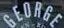
\includegraphics[width = 1.4in]{media/results/instances/gen-8.jpg}} &
        \subfloat{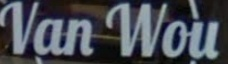
\includegraphics[width = 1.4in]{media/results/instances/gen-2.jpg}} \\
        \subfloat{
\includegraphics[width = 1.4in]{media/results/instances/gen-1.jpg}} &
        \subfloat{
\includegraphics[width = 1.4in]{media/results/instances/gen-4.jpg}} \\
    \end{tabular}
    \caption{Gentrified text instances examples}
    \label{fig:gen_sample}
\end{figure}

\begin{figure}
    \begin{tabular}{cccc}
        \subfloat{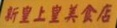
\includegraphics[width = 1.4in]{media/results/instances/non-gen-2.jpg}} &
        \subfloat{
\includegraphics[width = 1.4in]{media/results/instances/non-gen-1.jpg}} \\
        \subfloat{
\includegraphics[width = 1.4in]{media/results/instances/non-gen-3.jpg}} &
        \subfloat{
\includegraphics[width = 1.4in]{media/results/instances/non-gen-4.jpg}} \\
    \end{tabular}
    \caption{Non-gentrified text instances examples}
    \label{fig:nongen_sample}
\end{figure}


\subsection{Classification}
\subsubsection{Baseline}
Test set results of the baseline model are shown in Table \ref{fig:baseline_metrics}. 

\begin{table}[h]
\begin{tabular}{llcc}
\toprule
\multirow{2}{*}{Metrics}   & \multirow{2}{*}{Class} & \multicolumn{2}{c}{Baseline model}        \\ \cline{3-4} 
                           &                        & Classwise & Average                 \\ \hline
Accuracy                   & Gentrified             & 0.2143    & \multirow{2}{*}{0.5810} \\
                           & Non-gentrified         & 0.9478    &                         \\
Precision                  & Gentrified             & 0.6122    & \multirow{2}{*}{0.6852} \\
                           & Non-gentrified         & 0.7582    &                         \\
Recall                     & Gentrified             & 0.2143    & \multirow{2}{*}{0.5810} \\
                           & Non-gentrified         & 0.9478    &                         \\
F1-score                   & Gentrified             & 0.3175    & \multirow{2}{*}{0.5800} \\
                           & Non-gentrified         & 0.8425    &                         \\
\bottomrule
\end{tabular}
\caption{Test set classwise and macro-averaged metrics of baseline model (ResNet50, no weighted sampling, no fine-tuning). This model achieved very high performance for non-gentrified signage, but performed poorly on gentrified signage, due to class imbalance.}
\label{fig:baseline_metrics}
\end{table}


\subsubsection{Fine-tuned}
The best performing model with ResNet18 architecture was found with learning rate set to 0.001, batch size 32, and 60 training epochs. The best performing model with ResNet50 architecture was found with learning rate set to 0.01, batch size 64, and 60 training epochs. The macro-averaged metrics across classes for these models are shown in Table \ref{fig:resnet_compare}. The fine-tuned ResNet50 had better performance, its classwise metrics are shown in Table \ref{fig:resnet50_cls}.

\begin{table}[h!]
    \begin{tabular}{lcccc}
    \toprule
\multirow{2}{*}{Metrics} & \multicolumn{2}{c}{ResNet18} & \multicolumn{2}{c}{ResNet50} \\ \cmidrule(lr){2-3} \cmidrule(lr){4-5}
                         & Val           & Test          & Val           & Test         \\ \hline
Accuracy                 & 0.6497        & 0.6960        & 0.6506        & \textbf{0.7033}       \\
Precision                & 0.6185        & 0.6715        & 0.6209        & \textbf{0.6795}       \\
Recall                   & 0.6497        & 0.6960        & 0.6506        & \textbf{0.7033}       \\
F1-score                 & 0.6222        & 0.6781        & 0.6256        & \textbf{0.6865}       \\ \bottomrule
    \end{tabular}
    \caption{Macro-averaged metrics of the best-performing fine-tuned ResNet18 and ResNet50. Between these two models, the fine-tuned ResNet50 performed better.}
    \label{fig:resnet_compare}
\end{table}


\begin{table}[h!]
\begin{tabular}{llcc}
\toprule
\multirow{2}{*}{Metrics}   & \multirow{2}{*}{Class} & \multicolumn{2}{c}{ResNet50} \\ \cline{3-4} 
                           &                        & Val           & Test         \\ \hline
Accuracy                   & Gentrified             & 0.5714        & 0.6429       \\
                           & Non-gentrified         & 0.7299        & 0.7637       \\
Precision                  & Gentrified             & 0.3953        & 0.5114       \\
                           & Non-gentrified         & 0.8464        & 0.8476       \\
Recall                     & Gentrified             & 0.5714        & 0.6429       \\
                           & Non-gentrified         & 0.7299        & 0.7637       \\
F1-score                   & Gentrified             & 0.4674        & \textbf{0.5696}       \\
                           & Non-gentrified         & 0.7838        & \textbf{0.8035}       \\
\bottomrule
\end{tabular}
\caption{Classwise metrics of best model (fine-tuned ResNet50). Even though there was clear improvements in classifying gentrified signage compared to the baseline model, this model still did better on non-gentrified signage - most notably shown in the F1-scores of each class.}
\label{fig:resnet50_cls}
\end{table}

\subsection{Testing on extended data}
The average and classwise metrics of the best model in classifying the extended data are presented in Table \ref{fig:resnet50_pano}.

\begin{table}[h!]
\begin{tabular}{llcc}
\toprule
\multirow{2}{*}{Metrics}   & \multirow{2}{*}{Class} & \multicolumn{2}{c}{Extended data}   \\ \cline{3-4} 
                           &                        & Classwise & Average                 \\ \hline
Accuracy                   & Gentrified             & 0.5340    & \multirow{2}{*}{0.5807} \\
                           & Non-gentrified         & 0.6274    &                         \\
Precision                  & Gentrified             & 0.7359    & \multirow{2}{*}{0.5725} \\
                           & Non-gentrified         & 0.4092    &                         \\
Recall                     & Gentrified             & 0.5340    & \multirow{2}{*}{0.5807} \\
                           & Non-gentrified         & 0.6274    &                         \\
F1-score                   & Gentrified             & 0.6189    & \multirow{2}{*}{0.5571} \\
                           & Non-gentrified         & 0.4953    &                         \\
\bottomrule
\end{tabular}
\caption{Macro-average and classwise metrics of the best model in classifying the extended data. Compared to the metrics on StreetSwipe's test set, there was a consistent decrease of approximately 10\% in all average metrics on this data. Notably, this decrease mainly came from a worsened performance in classifying non-gentrified signage.}
\label{fig:resnet50_pano}
\end{table}


\subsection{Model prediction visualization}

\subsubsection{Correct classifications}

\begin{figure*}[]
    \centering
    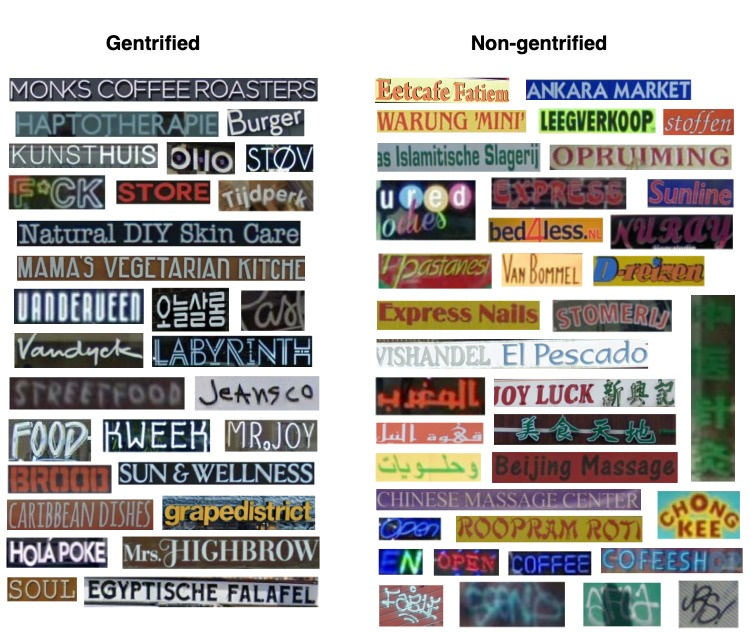
\includegraphics[width=0.8\textwidth]{media/results/output_vis.jpg}
    \caption{StreetSwipe's correctly classified signage per class with probability of 80\% and above. Note how non-gentrified signage varied more in their characteristics while gentrified signage appeared more homogenized. Non-gentrified signage used more colors, font types, and are largely in Dutch with appearances of English, Chinese, and Arabic. Gentrified signage vary less in font types and colors, and a lot of the instances are in English, with rare instances of non-Latin scripts (e.g. Korean).}
    \label{fig:output_vis}
\end{figure*}

StreetSwipe's signage per class with classification probability of 80\% and above were inspected. This showed the most typical and distinguishing characteristics of signage per class, which can be seen in Figure \ref{fig:output_vis}.

Gentrified signage were more similar in font types and often did not vary in text sizes, while non-gentrified signage used more types of fonts, sometimes more than one fonts on a single sign, and sometimes with varying text sizes and orientations. In addition, gentrified signs mostly had white texts, with minimal variation in background colors. Non-gentrified signs were the opposite: texts varied more in colors, as well as the background colors; and the appearance of neon signage in this class was also notable. In terms of languages, gentrified signage have more English text, with very rare appearances of non-Latin languages (e.g. Korean), while non-gentrified ones are largely in Dutch, with appearances of some English, Chinese and Arabic. And finally, although out of scope of the study, the model also picked up graffiti as instances belonging to non-gentrified facades.


\subsubsection{Incorrect classifications} 

\begin{figure*}[h!]
    \centering
    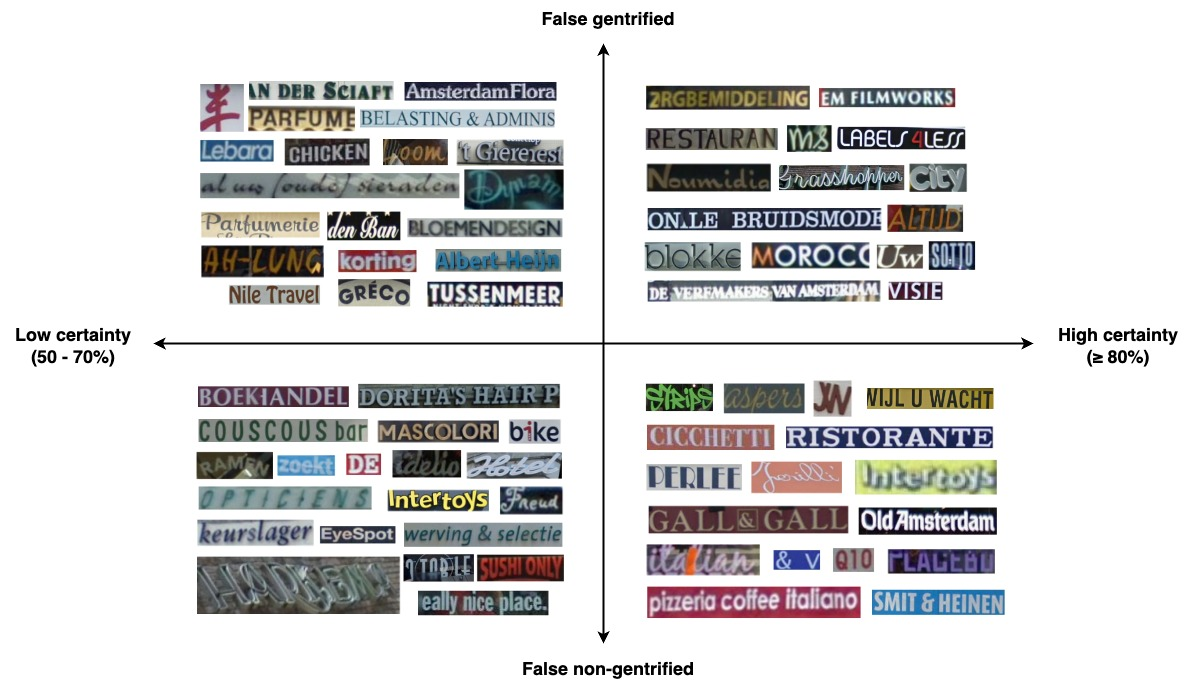
\includegraphics[width=0.9\textwidth]{media/results/output_vis-SS_incorrect.jpg}
    \caption{StreetSwipe's incorrectly classified signage per class, visualized by high and low classification certainty. Incorrect classifications with high certainty from both classes generally had the same characteristics as correctly classified instances (gentrified signage: mainly white text, less variation in font styles and background colors; non-gentrified signage: more variation in fonts, text colors and background colors). These signals diminished as classification certainty decreased: variations in fonts and colors were no longer distinctive across the two classes.}
    \label{fig:output_vis_SS_incorrect}
\end{figure*}

StreetSwipe's mis-classified signage per class with low (50-70\%) and high ($ \geq 80\% $) classification probabilities were inspected. The mis-classified instances with high certainty showed similar characteristics to correctly classified instances (gentrified signage: mainly white text, less variation in font styles and background colors; non-gentrified signage: more variation in fonts, text colors and background colors). On the other hand, mis-classified instances with lower certainty showed a more nuanced picture, whereby if distinguishing features per class appear together in one signage (e.g. non-white text (typical of non-gentrified) on white or dark background (typical of gentrified), signal strength diminished and the model's outputs of the two classes are less obviously distinguishable. Results can be seen in Figure \ref{fig:output_vis_SS_incorrect}.




\subsubsection{Classifications on extended data}

\begin{figure}[h!]
    \centering
    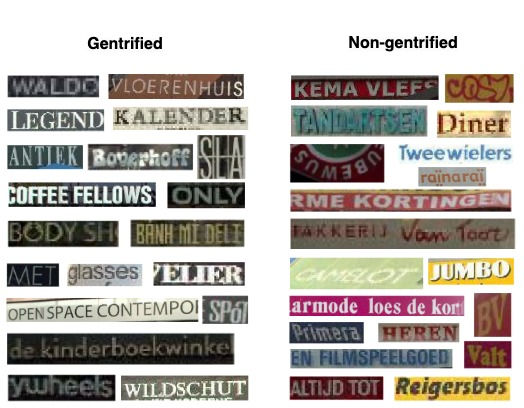
\includegraphics[width=0.45\textwidth]{media/results/output_vis-pano.jpg}
    \caption{Model's classifications on the extended data's signage with classification probability of 80\% and above (disregarding ground truth label). It's notable how the model's inference on this data showed the same characteristics per class as in StreetSwipe.}
    \label{fig:output_vis_pano}
\end{figure}

Model's classifications on the extended data's signage with classification probability of 80\% and above were inspected (disregarding ground truth label). Signage classified per class followed the same characteristics learned from StreetSwipe. Results can be seen in Figure \ref{fig:output_vis_pano}.


